\section{Fit optical potentials for elastic scattering of a nucleon on $^{208}$Pb target}
In this section we will do $\chi^2$ data fitting to obtain optical potentials 
for the elastic scattering of a proton or neutron on $^{208}$Pb. 
Experimental data are taken from Ref. \cite{MANI1971384_ProtonPb208Data} for proton and 
and \cite{PhysRevC.85.024619_NeutronPb208Data} for neutron. 
The beam energies of proton and neutron are 49.35 MeV and 40.0 MeV, respectively. 
In addition, we choose the optical parameters employed in Sec. \ref{part1} (Ref. \cite{capote2009ripl,koning2003local}) 
as the starting point of our fitting. 
All the results discussed in this section are generated by SFRESCO (Ref. \cite{FRESCO}). 

\subsection{Fit process and results}
All the intermediate and final results of our fitting are summarized in Table \ref{proton_table} (for proton) and Table \ref{neutron_table} (for neutron). 
For simplicity, we neglect spin-orbit components at the beginning, and only volume real and volume imaginary components are included. 
Keeping the volume imaginary component unchanged, we fit the volume real part (index 2 in Table \ref{proton_table} and \ref{neutron_table}), 
which cannot reduce $\chi^2/N$ to a low value. 
Then, we vary both volume real and imaginary parts simultaneously (index 3 in Table \ref{proton_table} and \ref{neutron_table}) and 
achieve a significant improvement.  
However, for proton the diffuseness parameter av becomes too small to be considered physical. 
\par
Another choice of optical potential is to use a surface imaginary component instead of a volume one. 
Starting from parametrization of index 4 in Table \ref{proton_table} and \ref{neutron_table}, we fit the volume real part and surface imaginary part 
(index 5 in Table \ref{proton_table} and \ref{neutron_table}). 
For both proton and neutron, a surface imaginary component gives a lower $\chi^2/N$, 
and thus we will add spin-orbit terms onto this optical potential form. 
\par
As shown in the last four lines in Table \ref{proton_table} and \ref{neutron_table}, 
we gradually add and fit different parameters in the spin-orbit term.  
As for proton, the description can hardly be improved by only adding a real spin-orbit potential (index 6 in Table \ref{proton_table}).  
If we only add a imaginary spin-orbit component, the diffuseness parameter ``awso" will become negative and thus unphysical 
(index 8 in Table \ref{proton_table}), so we abandon this set of parameters. 
If both real and imaginary components of spin-orbit potential are included, $\chi^2/N$ will slightly decrease from 4.860 to 3.611,
(index 9 in Table \ref{proton_table}), which indicates that the spin-orbit term is not very important 
for the description of elastic scattering of a proton on $^{208}$Pb. 
\par
As for neutron, the radius parameter ``rvso'' will become negative and unphysical when only a real spin-orbit component is included 
(index 6 in Table \ref{neutron_table}), so we abandon this set of parameters. 
By only adding an imaginary spin-orbit component, $\chi^2/N$ is slightly lowered from 4.638 to 3.310 
(index 8 in Table \ref{neutron_table}). 
When both real and imaginary spin-orbit parts are varied, $\chi^2/N$ can be even lower (index 9 in Table \ref{neutron_table}). 
But in this case the diffuseness ``avso" will become less than radius ``rvso", which is unphysical and unacceptable. 
As no significant improvement is seen from adding spin-orbit terms, we think that 
the spin-orbit term is not important for the description of elastic scattering of a neutron on $^{208}$Pb. 

\begin{landscape}
	\begin{table}[t]
		\centering
		\caption{Fitting results of scattering of a proton on $^{208}$Pb. 
		The unit of Vv, Wv, Ws, Vso and Wso is MeV, and the unit of rv, av, rwv, awv, rws, aws, rvso, avso, rwso and awso is fm. 
	    Unphysical values are highlighted in red. }
		\label{proton_table}
		\footnotesize
		\begin{tabular}{cccccccccccccccccc}
			\hline
			\hline
			Index & Fit from & Vv  & rv  & av  & Wv & rwv & awv  & Ws & rws & aws & Vso & rvso & avso & Wso & rwso & awso & $\chi^2/N$ \\
			\hline
			1     & -          & 67.2     & 1.244   & 0.646    & 16.6     & 1.244    & 0.646    & -        & -        & -        & -         & -         & -         & -         & -         & -        & 78.285   \\
			2     & 1          & 46.1     & 1.262   & 0.574    & 16.6     & 1.244    & 0.646    & -        & -        & -        & -         & -         & -         & -         & -         & -        & 27.134   \\
			3     & 2          & 44.6     & 1.254   & 1.87E-04 & 4.89     & 1.726    & 0.171    & -        & -        & -        & -         & -         & -         & -         & -         & -        & 5.479    \\
			4     & -          & 46.1     & 1.262   & 0.574    & -        & -        & -        & 19.5     & 1.246    & 0.615    & -         & -         & -         & -         & -         & -        & 11.335   \\
			5     & 4          & 45.3     & 1.229   & 0.528    & -        & -        & -        & 13.2     & 1.295    & 0.713    & -         & -         & -         & -         & -         & -        & 4.860    \\
			6     & 5          & 45.2     & 1.232   & 0.489    & -        & -        & -        & 12.7     & 1.295    & 0.732    & 0.14     & 1.07     & 0.55     & -         & -         & -        & 4.838    \\
			7     & -          & 45.2     & 1.232   & 0.489    & -        & -        & -        & 12.7     & 1.295    & 0.732    & -         & -         & -         & -3.1    & 1.08      & 0.57     & 12.026   \\
			8     & 7          & 45.1     & 1.242   & 0.507    & -        & -        & -        & 12.0     & 1.279    & 0.748    & -         & -         & -         & -2.1     & 0.66     & \color{red}{-0.028}   & 4.068    \\
			9     & 7          & 45.2     & 1.276   & 0.540    & -        & -        & -        & 15.7     & 1.239    & 0.710    & -6.9     & 0.84     & 0.55     & -8.0     & 1.03      & 0.53     & 3.661   \\
			\hline
			\hline
		\end{tabular}
	\end{table}

\begin{table}[b]
	\centering
	\caption{Fitting results of scattering of a neutron on $^{208}$Pb. 
			The unit of Vv, Wv, Ws, Vso and Wso is MeV, and the unit of rv, av, rwv, awv, rws, aws, rvso, avso, rwso and awso is fm. 
			Unphysical values are highlighted in red. }
	\label{neutron_table}
	\footnotesize
	\begin{tabular}{cccccccccccccccccc}
		\hline
		\hline
		index & Fit from & Vv   & rv    & av    & Wv    & rwv   & awv   & Ws   & rws   & aws   & Vso & rvso  & avso & Wso   & rwso & aso  & $\chi^2/N$ \\
		\hline
		1     & -        & 50.6 & 1.244 & 0.646 & 15.6  & 1.244 & 0.646 & -    & -     & -     & -   & -     & -    & -     & -    & -    & 261.394    \\
		2     & 1        & 40.3 & 1.245 & 0.903 & 15.6  & 1.244 & 0.646 & -    & -     & -     & -   & -     & -    & -     & -    & -    & 46.553     \\
		3     & 2        & 41.9 & 1.154 & 0.762 & 6.598 & 1.383 & 0.824 & -    & -     & -     & -   & -     & -    & -     & -    & -    & 7.900      \\
		4     & -        & 40.3 & 1.245 & 0.903 & -     & -     & -     & 13.8 & 1.246 & 0.510 & -   & -     & -    & -     & -    & -    & 98.423     \\
		5     & 4        & 36.4 & 1.269 & 0.585 & -     & -     & -     & 14.4 & 1.097 & 0.500 & -   & -     & -    & -     & -    & -    & 4.638      \\
		6     & 5        & 36.1 & 1.277 & 0.578 & -     & -     & -     & 15.7 & 1.108 & 0.498 & 8.3 & \color{red}{-4.3} & 3.2 & -     & -    & -    & 3.084      \\
		7     & -        & 36.4 & 1.269 & 0.585 & -     & -     & -     & 14.4 & 1.097 & 0.500 & -   & -     & -    & -3.1 & 1.08 & 0.57 & 35.163     \\
		8     & 7        & 36.4 & 1.273 & 0.593 & -     & -     & -     & 15.2 & 1.109 & 0.519 & -   & -     & -    & -3.1 & 1.09 & 0.43 & 3.310      \\
		9     & 8        & 35.8 & 1.266 & 0.592 & -     & -     & -     & 14.9 & 1.107 & 0.513 & 4.9 & \color{red}{1.03}  & \color{red}{1.23} & -3.0 & 1.06 & 0.81 & 2.258      \\
		\hline
		\hline
	\end{tabular}
\end{table}
\end{landscape}

\subsection{Fit Sensitivity to Initialization}
Here we study the sensitivity of SFRESCO fitting to initial parameters. We used volume real and surface imaginary components of the optical potential only. Although there is improvement in the neutron scattering fit by inclusion of a spin-orbit imaginary term, optimal fits without this term are roughly 40\% of the fit with this additional term ($\chi^2/N = 3.310, 4.638 $). Optimal initial parameters were determined by successive fitting and reinitializing output parameters until a stable minimum was achieved with parameters comparable to the initial global potential fits from \cite{capote2009ripl}.
\par
In Figure \ref{fig:initializations} below, we plot the SFRESCO $\chi^2/N$ fit error against modifications of a single parameterization. To overlay dissimilar parameter values, the plotted input parameter is normalized by its determined optimized value. $\chi^2/N$ as a choice of parameter of interest (as opposed to the output value of the varied parameter) was from the observation that  $\chi^2/N$ correlates strongly with optical potential parameters approaching the optimal fit values within a few percent. From Fig \ref{fig:pnV}, we see that initializations to both depth parameters for protons and neutrons arrive at optimum for roughly $\pm$50\% of optimal values. From Fig. \ref{fig:pnr}, While not as centered around $\frac{P_{in}}{P_{optimal}}=1$ as the depth parameters, the radius parameters appear to converge for roughly $\pm$25\% of optimal values. In Fig. \ref{fig:pna}, we demonstrate that diffuseness is potentially the most convergent parameter (see neutron surface imaginary converge for $\pm$100\% of the optimal value), diffuseness is the least consistent parameter. The worst demonstrated convergence is the proton surface imaginary diffuseness, which converges for $\frac{P_{in}}{P_{optimal}}=1.0-0.0+0.5$.
\par
Two peculiarities were discovered while spanning these parameters.
\begin{enumerate}
	\item Multiple initializations regions of the proton real volume depth lead to optimal parameterization. Fig. \ref{fig:pnV} shows how $V_0\approx 0$ gives results consistent with $V_0 \approx V_{optimal}$ while the region $0.1 \leq \frac{V_0}{V_{optimal}} \leq 0.6$ returns a significantly worse fit.
	\item There appears to be a numerical instability for the neutron real volume depth $\frac{V_0}{V_{optimal}} = 0.55 \pm <0.05$. This instability sits in a region of efficient optimal parameter finding, and has width of $<$ 3 MeV. Given the approximate nature of the global potentials that were used to arrive at optimal fitting parameters, this narrow instability is concerning and so a range of initial values (centered around the global parameter fit) ought to be considered. 
\end{enumerate}
\begin{figure}[h]
	\begin{subfigure}{0.5\textwidth}
		
		\centering
		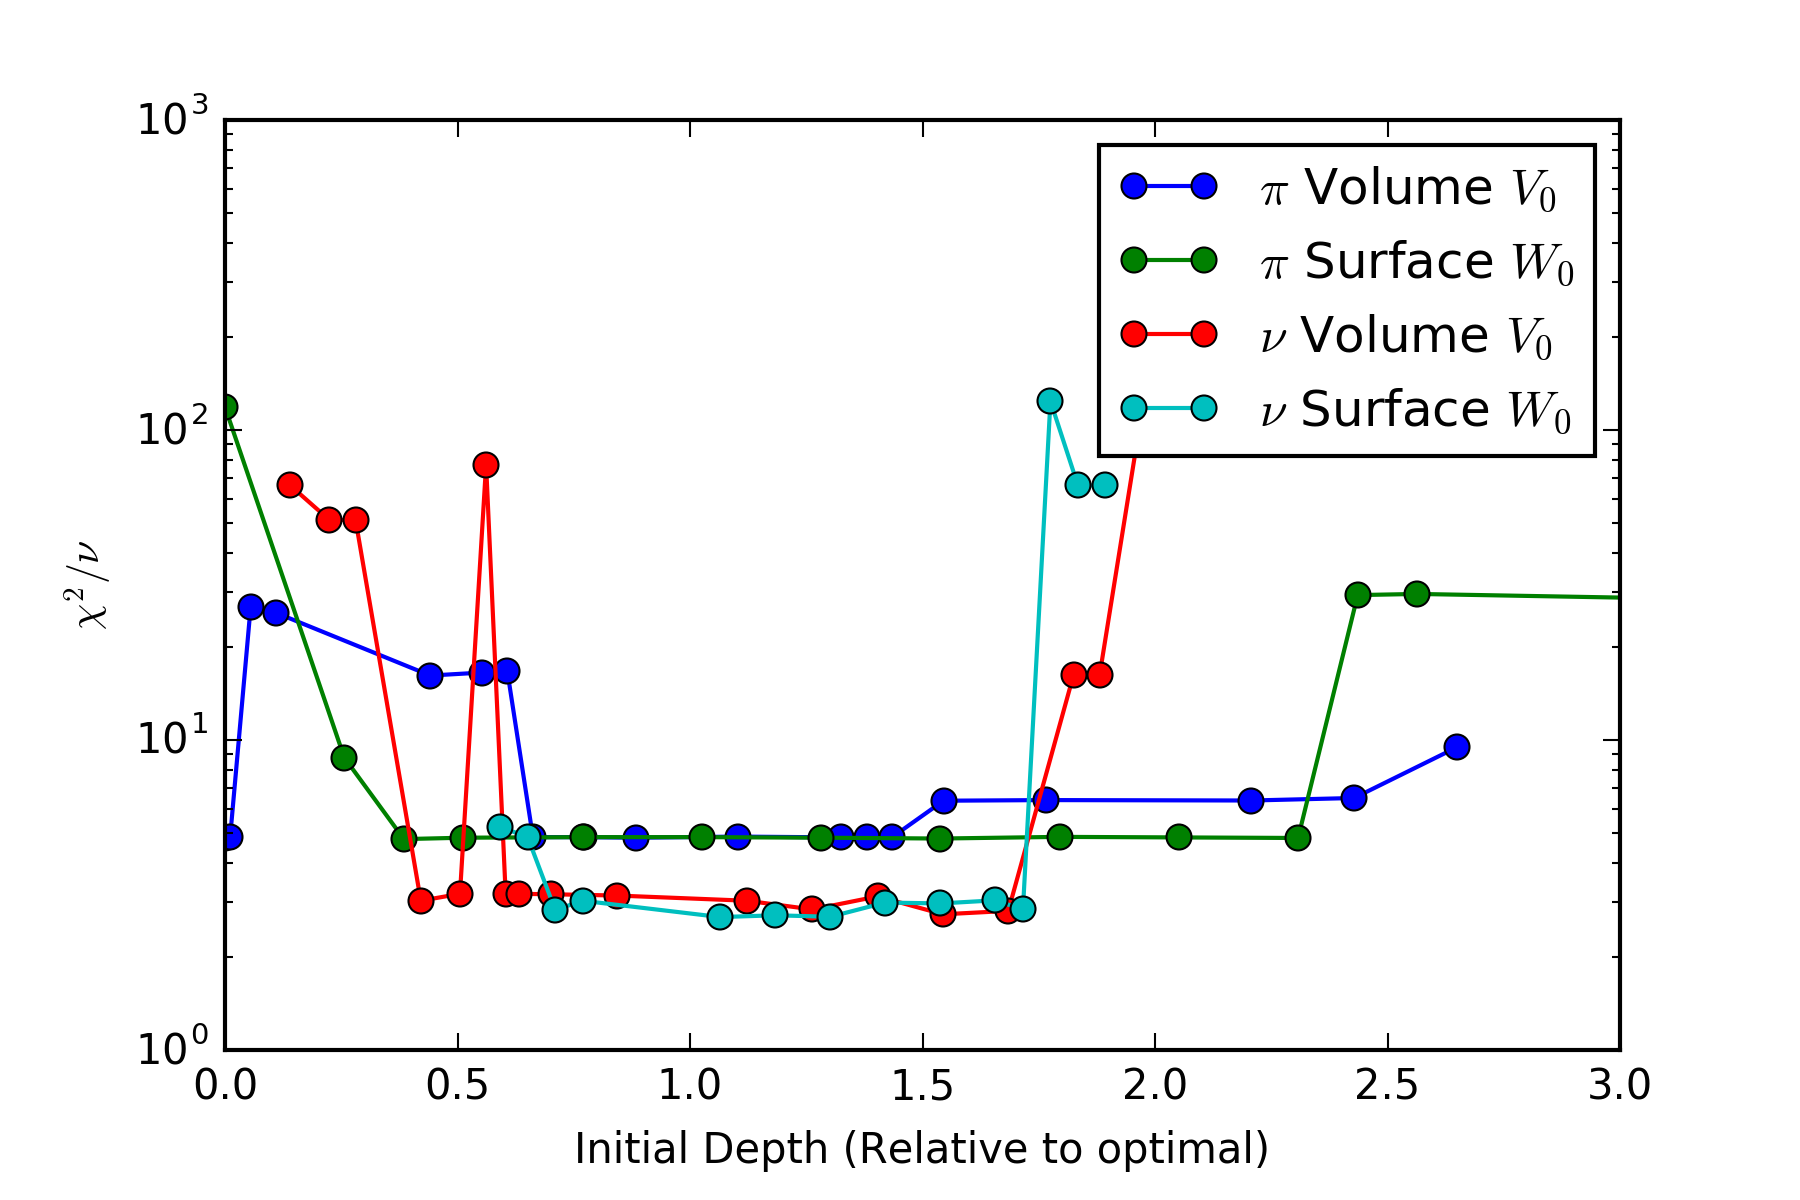
\includegraphics[width=0.98\textwidth]{pnV.png}
		\caption{Optical potential depth parameters }
		\label{fig:pnV}
	\end{subfigure}
	\begin{subfigure}{0.5\textwidth}
		\centering
		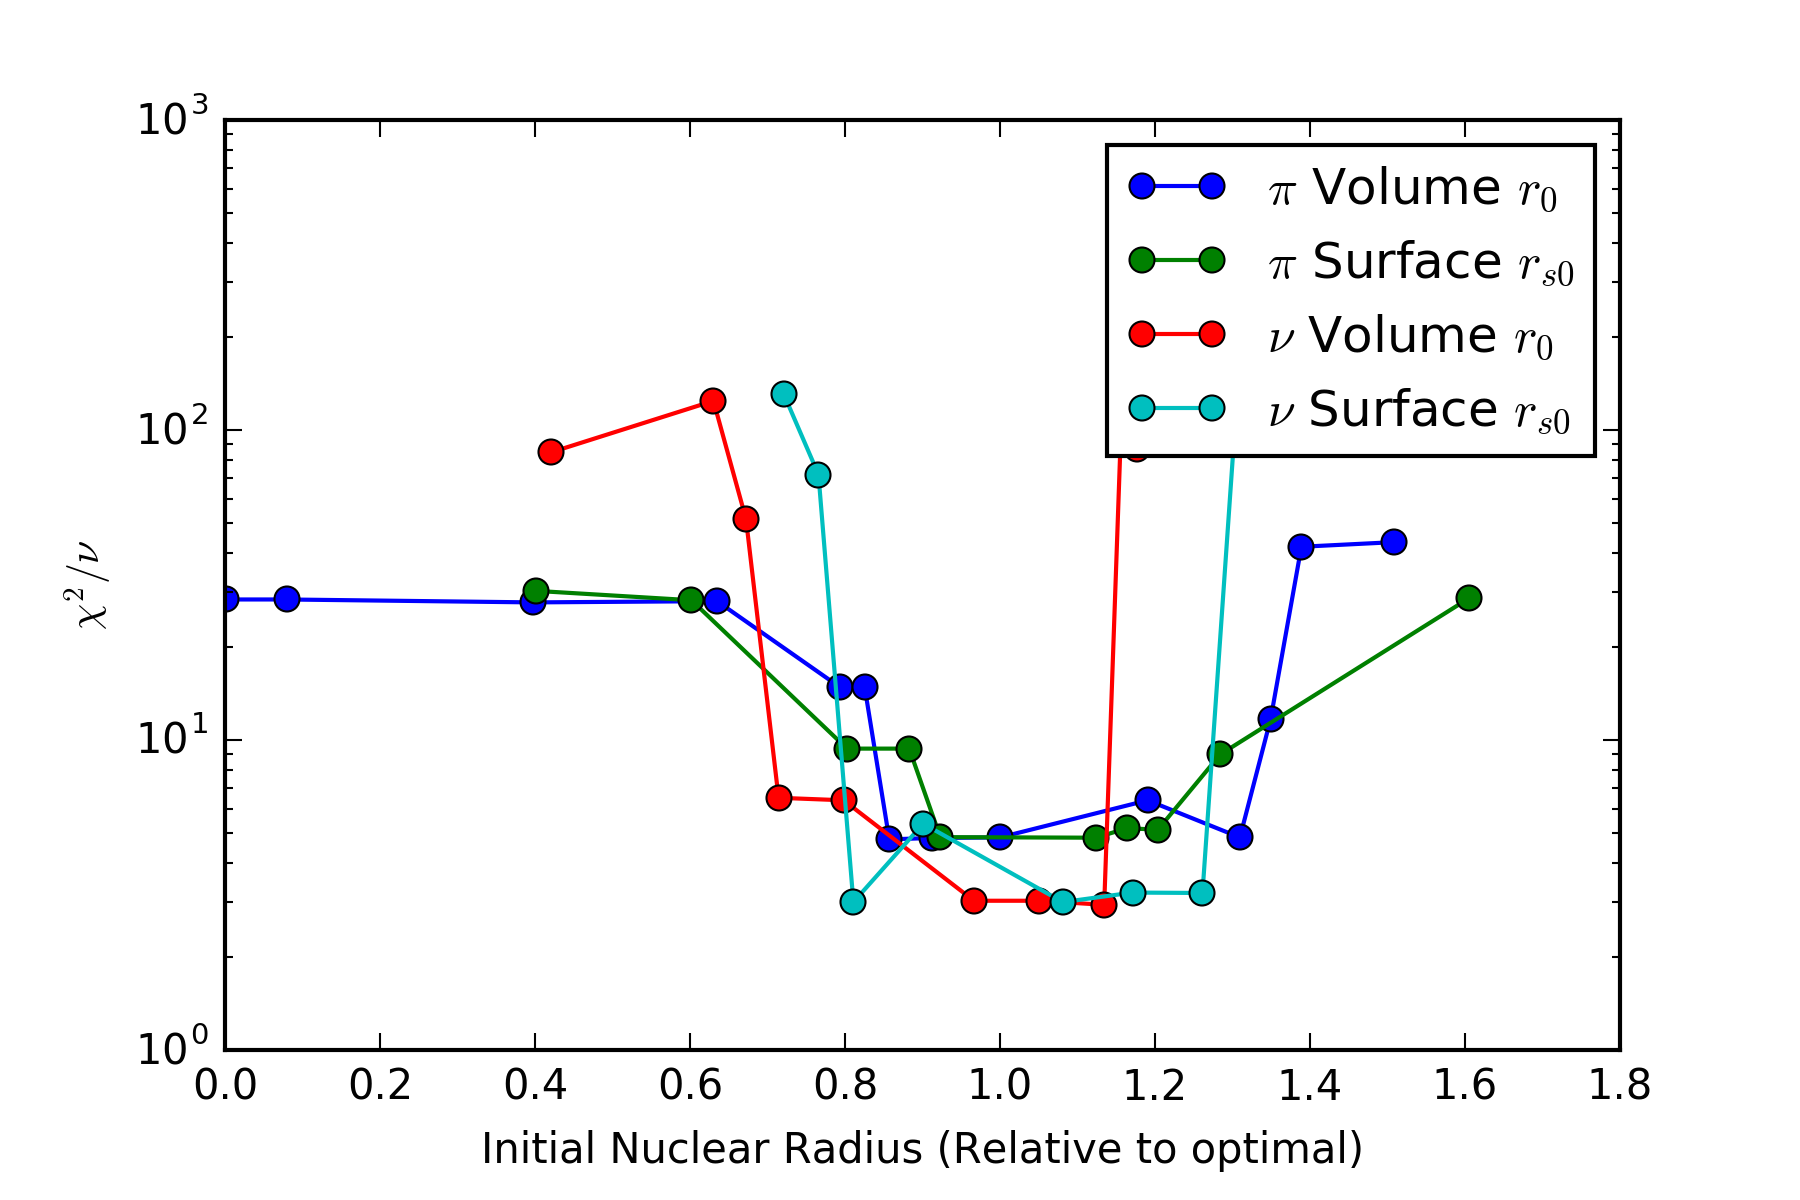
\includegraphics[width=0.98\textwidth]{pnr.png}
		\caption{Nuclear radius parameters }
		\label{fig:pnr}
	\end{subfigure}
	\begin{subfigure}{0.5\textwidth}
		\centering
		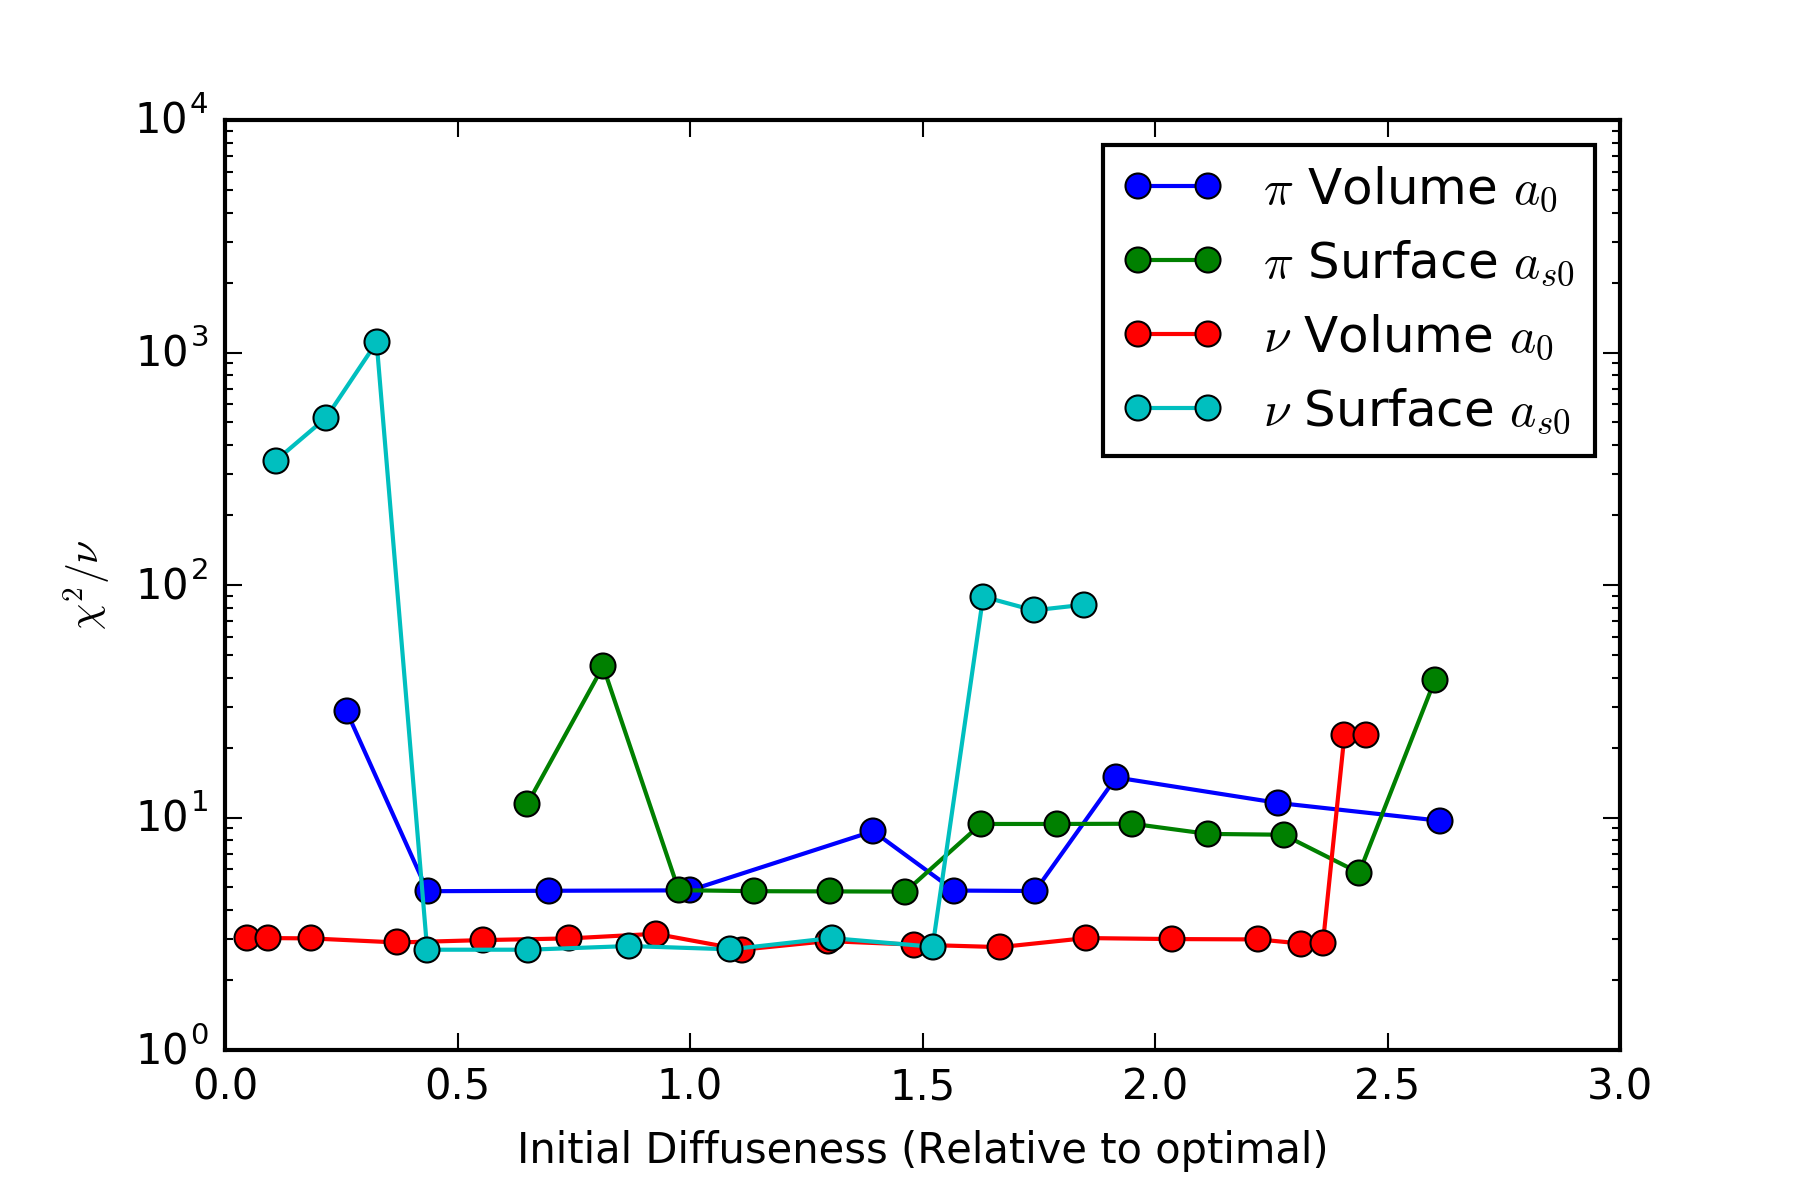
\includegraphics[width=0.98\textwidth]{pna.png}
		\caption{Nuclear diffuseness parameters  }
		\label{fig:pna}
	\end{subfigure}
	\caption{Measure of error of SFRESCO fits for different initial parameterization of the depth part of the optical potential for 49.35 MeV protons ($\pi$) and 40 MeV neutrons ($\nu$) scattering on $^{208}$Pb. Plotted on the x-axis is the ratio of $\frac{P_{initial}}{P_{optimal}}$. }
	\label{fig:initializations}
\end{figure}